\section{Overview}

\begin{figure*}
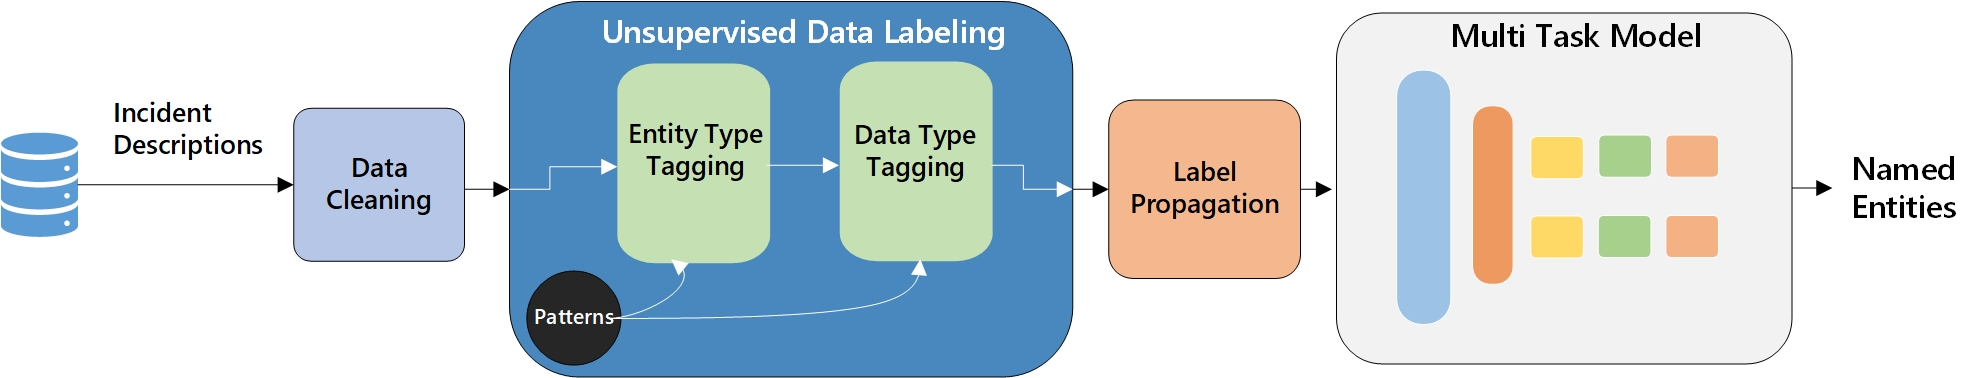
\includegraphics[width=1\textwidth]{Figures/System_Architecture_Diagram.jpg}
\caption{Machine learning pipeline}
\label{fig:overview}
%\vspace{-6pt}
\end{figure*}

Incident management is key to running large scale services in an efficient and performant way. However, there is a lot of scope for optimization which can increase customer satisfaction, reduce on-call fatigue and provide revenue savings. Existing work on incident management has focused on specific problems such as incident triaging. The state of the art incident triaging methods \cite{ContinuousTriageASE2019} use novel deep learning methods which takes the unstructured incident description, discussions and title, and predict the team to which the incident should be triaged. In this work, we focus on the fundamental problem of structured knowledge extraction from these unstructured incidents. With the structured information, not only can we build machine learning models for tasks like triaging, but we can also save a lot of time and effort for on-call engineers by automating the manual processes such as running health checks on resources.

To solve the challenges with incident management, we have designed the \softner{} framework. It is the first automated approach for structured knowledge extraction from service incidents. We frame the knowledge extraction problem as a \textit{Named-Entity Recognition} (NER) task which has been well explored in the Information Retrieval (IR) domain \cite{nadeau2007survey, lample2016neural}. Named-Entity Recognition is defined as the task of parsing unstructured text to not only detect entities but also classify them into specific categories. An entity can be any chunk of text which belongs to a given type or category. For example, in the IR domain, some of the most commonly used entity types are people, locations and organizations. As an example, here is the input and output of a NER task for a news headline:

\smallskip%\medskip
\textit{\textbf{Input}}: Over 320 million people have visited the Disneyland in Paris since it opened in 1992.

\smallskip
\textit{\textbf{Output}}: Over \textbf{[\textsubscript{COUNT} 320 million]} people have visited the \textbf{[\textsubscript{ORG} Disneyland]} in \textbf{[\textsubscript{LOC} Paris]} since it opened in \textbf{[\textsubscript{YEAR} 1992]}.

\smallskip%\medskip

Framing the knowledge extraction problem as a NER task enables us to not only extract factual information from the incidents but also classify them as specific entities. For instance, if we just extract a \textit{GUID} from the text, it provides limited context. However, identifying that \textit{GUID} as a \textit{Subscription Id} is much more useful. Figure \ref{fig:overview} provides an overview of the various components of the \softner{} framework. In this framework we combine techniques from the information retrieval and the deep learning domains for solving the problem of knowledge extraction. One key limitation of any machine learning based pipeline is the requirement of huge amounts of labeled data which can be cost prohibitive to manually generate. In service incidents, the lack of existing training data prevents us from using any supervised or semi-supervised techniques.

\softner{} uses pattern extractors which leverage the \emph{key-value} and \emph{tabular} structural patterns in the incident descriptions to bootstrap the training data. We then use label propagation to generalize the training data beyond these patterns. Then we design a novel Multi-Task deep learning model which is able to extract named-entities from the unstructured incident descriptions with very high accuracy. The model not only leverages the semantic features but also the data type of the individual tokens (such as GUID, URI, Boolean, Numerical, IP Address etc.). Below we list some of the terms which we will be using throughout the rest of the paper. These terms identify different aspects of the named-entities.

\begin{itemize}
\item \textbf{Entity Name:} N-gram indicating the name of the entity. In the current implementation, N can range from 1 to 3. We also enforce the entity names to be alphabetical to filter out noisy data.
\item \textbf{Entity Value:} The value of the named-entity for a given instance. 
\item \textbf{Data Type:} The data type of the values for the named-entity.
\end{itemize} 

\textbf{Example}: Let's consider a real incident reported by a customer of the Cloud Networking service operated by \CompanyX{}. The incident was caused due to an error in deleting a Virtual Network resource. The key information required to triage and mitigate this incident is actually the `\textit{Problem Type}' and the `\textit{Virtual Network Id}'. This information is already present in unstructured form within the incident description, the challenge is to extract it automatically in a structured format. Using \softner{}, we can not only provide key information about the incidents to the on-call engineers, but, also automate some of the manual tasks such as running health checks. For instance, in the previous example, we can automatically look up the current status and logs before the on-call engineer engages. Lastly, the extracted knowledge can also be used to build more accurate machine learning models for predictive tasks like triaging, root causing, etc.